\documentclass[a4paper,doc,floatsintext,natbib]{apa6}
%% \documentclass{article}
\usepackage[font=large]{caption}
\usepackage{natbib}
\usepackage{graphicx}
\usepackage{amsmath}
\usepackage{amsfonts}
\usepackage[utf8]{inputenc}
\usepackage{nameref}
\usepackage{todonotes}
\usepackage{authblk}
% \usepackage[nomarkers,figuresonly]{endfloat}
\usepackage{multirow}
\usepackage{tabularx}

% Remember to start reftex-mode

\setlength{\parskip}{1em}
\def \fref #1{Figure \ref{#1}}     % Reference figures
\def \tref #1{Table \ref{#1}}      % Reference tables
\def \eref #1{Equation \ref{#1}}   % Reference equations
\def \sref #1{Section '\nameref{#1}'}    % Reference sections

\DeclareMathOperator*{\argmin}{argmin}
\DeclareMathOperator*{\argmax}{argmax}

% For revision
\DeclareRobustCommand{\newcontent}[1]{#1}

\title{The effects of probabilistic context inference on motor adaptation}
\shorttitle{Context-inference-dependent motor adaptation}
\author[1,2]{Cuevas Rivera, Darío}
\author[1,2]{Kiebel, Stefan J.}
\affil[1]{Chair of Neuroimaging, Faculty of Psychology, Technische Universität Dresden, 01062 Dresden, Germany.}
\affil[2]{Centre for Tactile Internet with Human-in-the-Loop (CeTI)}
% \author[1]{Author list}
% \affil[1]{Affiliation list}
\affiliation{~}

\begin{document}

\maketitle

\abstract{Abstract}
Humans have been shown to adapt their movements when sudden or gradual changes to the dynamics of the environment are introduced, a phenomenon called motor adaptation. If the change is reverted, the adaptation is also quickly reverted. Humans are also able to adapt to multiple changes in dynamics presented separately, and to be able to switch between adapted movements on the fly. Such switching relies on contextual information which is often noisy or misleading, which affects the switch between adaptations. Recently, the COIN computational model for motor adaptation and context inference was introduced, which contains explicit components of context inference and Bayesian motor adaptation. This model was used to show the effects of context inference on learning rates across different experiments. We expanded on that work by using the COIN model to show that the effects of context inference on motor adaptation and control go even further than previously shown. Here, we used the COIN model to simulate classical motor adaptation experiments from previous works and showed that context inference, and how it is affected by the presence and reliability of feedback, effect a host of behavioral phenomena that had so far required multiple hypothesized mechanisms, lacking a unified explanation. Concretely, we show that the reliability of direct contextual information, as well as noisy sensory feedback, typical of many experiments, effect measurable changes in switching-task behavior, as well as in action selection, that stem directly from probabilistic context inference. 


\section{Introduction}
It has been shown that humans can adapt motor commands to counteract changes in the dynamics of the environment and their own bodies, such as performing reaching movements with a weight attached to the wrist. This is known as motor adaptation. Moreover, human participants have been shown to adapt to different, even opposing, changes during the course of a single experiment \citep{Gandolfo_Motor_1996,Shadmehr_Functional_1997}. Additionally, humans have been shown to dynamically switch between different learned adaptations \citep{Davidson_Scaling_2004,Ethier_Spontaneous_2008,Lee_Dual_2009}.

By introducing blocks of trials in which body dynamics are altered (e.g. a mechanical arm exerts a force on the participant's hand), experimenters are able to observe motor adaptation through the lens of motor error. Across many different motor adaptation experiments \citep[e.g.][]{Gandolfo_Motor_1996,Shadmehr_Adaptive_1994,Davidson_Scaling_2004}, well-established phenomena have been observed: (i) the ability to recall previously-learned skills, called savings; (ii) the ability to return to unmodified dynamics, termed de-adaptation; (iii) the interference in motor learning between opposing manipulations in dynamics, called anterograde interference; (iv) spontaneous display of behavior consistent with a previously-learned adaptation, during trials where errors are forced to be zero, called spontaneous recovery.

To explain these phenomena, a number of computational models have been introduced, which adapt their motor commands after observing motor errors. The most studied are linear learners \citep{Smith_Interacting_2006,Forano_Timescales_2020,Scheidt_Learning_2001}, but Bayesian accounts have also been presented, providing an alternative explanation for savings and quick de-adaptation in the form of switching between forward models \citep{Kording_Bayesian_2004,Oh_Minimizing_2019}.

While these general models of adaptation explain the most common phenomena observed in experiments, other known phenomena remain outside of their scope. For example, it is known that adaptation rate is reduced in situations where the environment is unstable and unpredictable \citep{Herzfeld_memory_2014}, or situations in which errors are small \citep{Marko_Sensitivity_2012} or adaptations slowly introduced \citep{Huang_Persistence_2009}. Action selection has also been found to depend on the history of adaptations learned \citep{Vaswani_Decay_2013,Davidson_Scaling_2004}.

Recently, a new computational model for context-dependant motor learning based on Bayesian inference was introduced by \cite{Heald_Contextual_2021}, called COIN (for context inference). \cite{Heald_Contextual_2021} formalized context inference as a process that operates independently from motor learning, but is informed by it, establishing a loop whereby context inference also informs motor learning. With this model, \cite{Heald_Contextual_2021} showed that context inference causes the observed changes in the rate of motor learning in previous experiments \cite[e.g.][]{Herzfeld_Encoding_2018}.

In this work, we use the COIN model to show that the process of context inference underlies more behavioral phenomena than previously shown. We focused on the effects of uncertain contextual information on switching behavior, especially during so-called error-clamp trials, in which errors are forced to zero by experimenters. More specifically, we focused on the effects of perceptual noise, as well as feedback modalities, in context inference, which in turn affects behavior in ways that can be directly measured. We show that through context inference, switching behavior can display three main effects that have been previously attributed to hypothesized ad-hoc mechanisms: (1) The size of an adaptation dictates how quick and reliable switching between tasks is \cite{Oh_Minimizing_2019,Kim_Neural_2015}, which we explain in terms of the effects of perceptual noise on context inference. (2) Previously-learned adaptations can interfere with switching behavior \citep{Davidson_Scaling_2004}, which we explain in terms of uncertain context inference. (3) Training history (i.e. which adaptations have been learned and for how long) affects switching during error-clamp trials \citep{Vaswani_Decay_2013}, which we also attribute to uncertain context inference. To do this, we used the COIN model to simulate the experimental setups and the decision-making agents (i.e. participants) during those experiments.

With these combined simulations and their qualitative comparison to the experimental phenomena outlined, we provide further evidence that context inference may be a single coherent and mechanistic account that underlies experimentally well-established motor adaption and history effects under changing contexts.

\section{Results}
Using the COIN model \citep{Heald_Contextual_2021}, we simulated representative experiments from a number of experimental studies on motor adaptation to illustrate how this model explains different experimental findings using the dynamics of context inference. We will present these simulations alongside the experimental results from the representative studies and discuss in detail how context inference explains the experimental phenomena.

Before presenting these results, we briefly describe the COIN model, leaving a more thorough explanation for the methods section. Additionally, we present simulations using the model that show the effects of contextual cues and perceptual noise on context inference, which pave the way for the simulated experiments that we show later on.


\subsection{Modeling context-dependent adaptation}
We focused on three main components of the COIN model: (1) context inference, (2) motor adaptation and (3) action selection. The processes defined by these component occur in this order, and each component informs the ones that follow.

Central to the model is the concept of context, defined in terms of the task to be performed, the variables of the environment that are relevant to perform the task, the forward models used by the decision-making agent to perform the task, and the update mechanisms necessary to adapt these forward models to the changing environment. Together, these elements allow the agent to make predictions on future observations when this context is active, and these predictions are used to infer the context. For example, when lifting an object of unknown weight, an agent might have learned one context for heavy objects and one for light objects. When observing an object to be lifted, the agent can use its size and texture to estimate the weight of the object, which in turn allows the agent to infer the appropriate context and, with it, decide how to lift the object.

The COIN model contains, additionally to these three main components, components for learning new contexts (i.e. inferring the existence of a new context that had not been previously encountered by the agent), as well as the ability to infer subject-specific parameters such as a participant's assumed transition probabilities between contexts, which can differ from the real, hidden transition probabilities. In this work, we focus on switching behavior between previously-learned contexts, as well as in the perceptual aspect of context inference. Additionally, we do not fit the COIN model to participant data, instead focusing on showing the way the COIN model explains known experimental phenomena. For these reasons, we chose not to use these components of the COIN model, instead fixing both the transition probabilities between contexts and the number of contexts based on the real values during the experiments, which were made available to participants \todo{Check this}. Fixing these values, in turn, allowed us to simplify the generative model, internal to the agent, using conjugate priors, with which the agent can do exact Bayesian inference. The generative model we used here can be seen in \fref{fig:model}A, including the priors for both context inference and motor adaptation. For more details on these choices, see the Methods section.

\begin{figure}
\centering
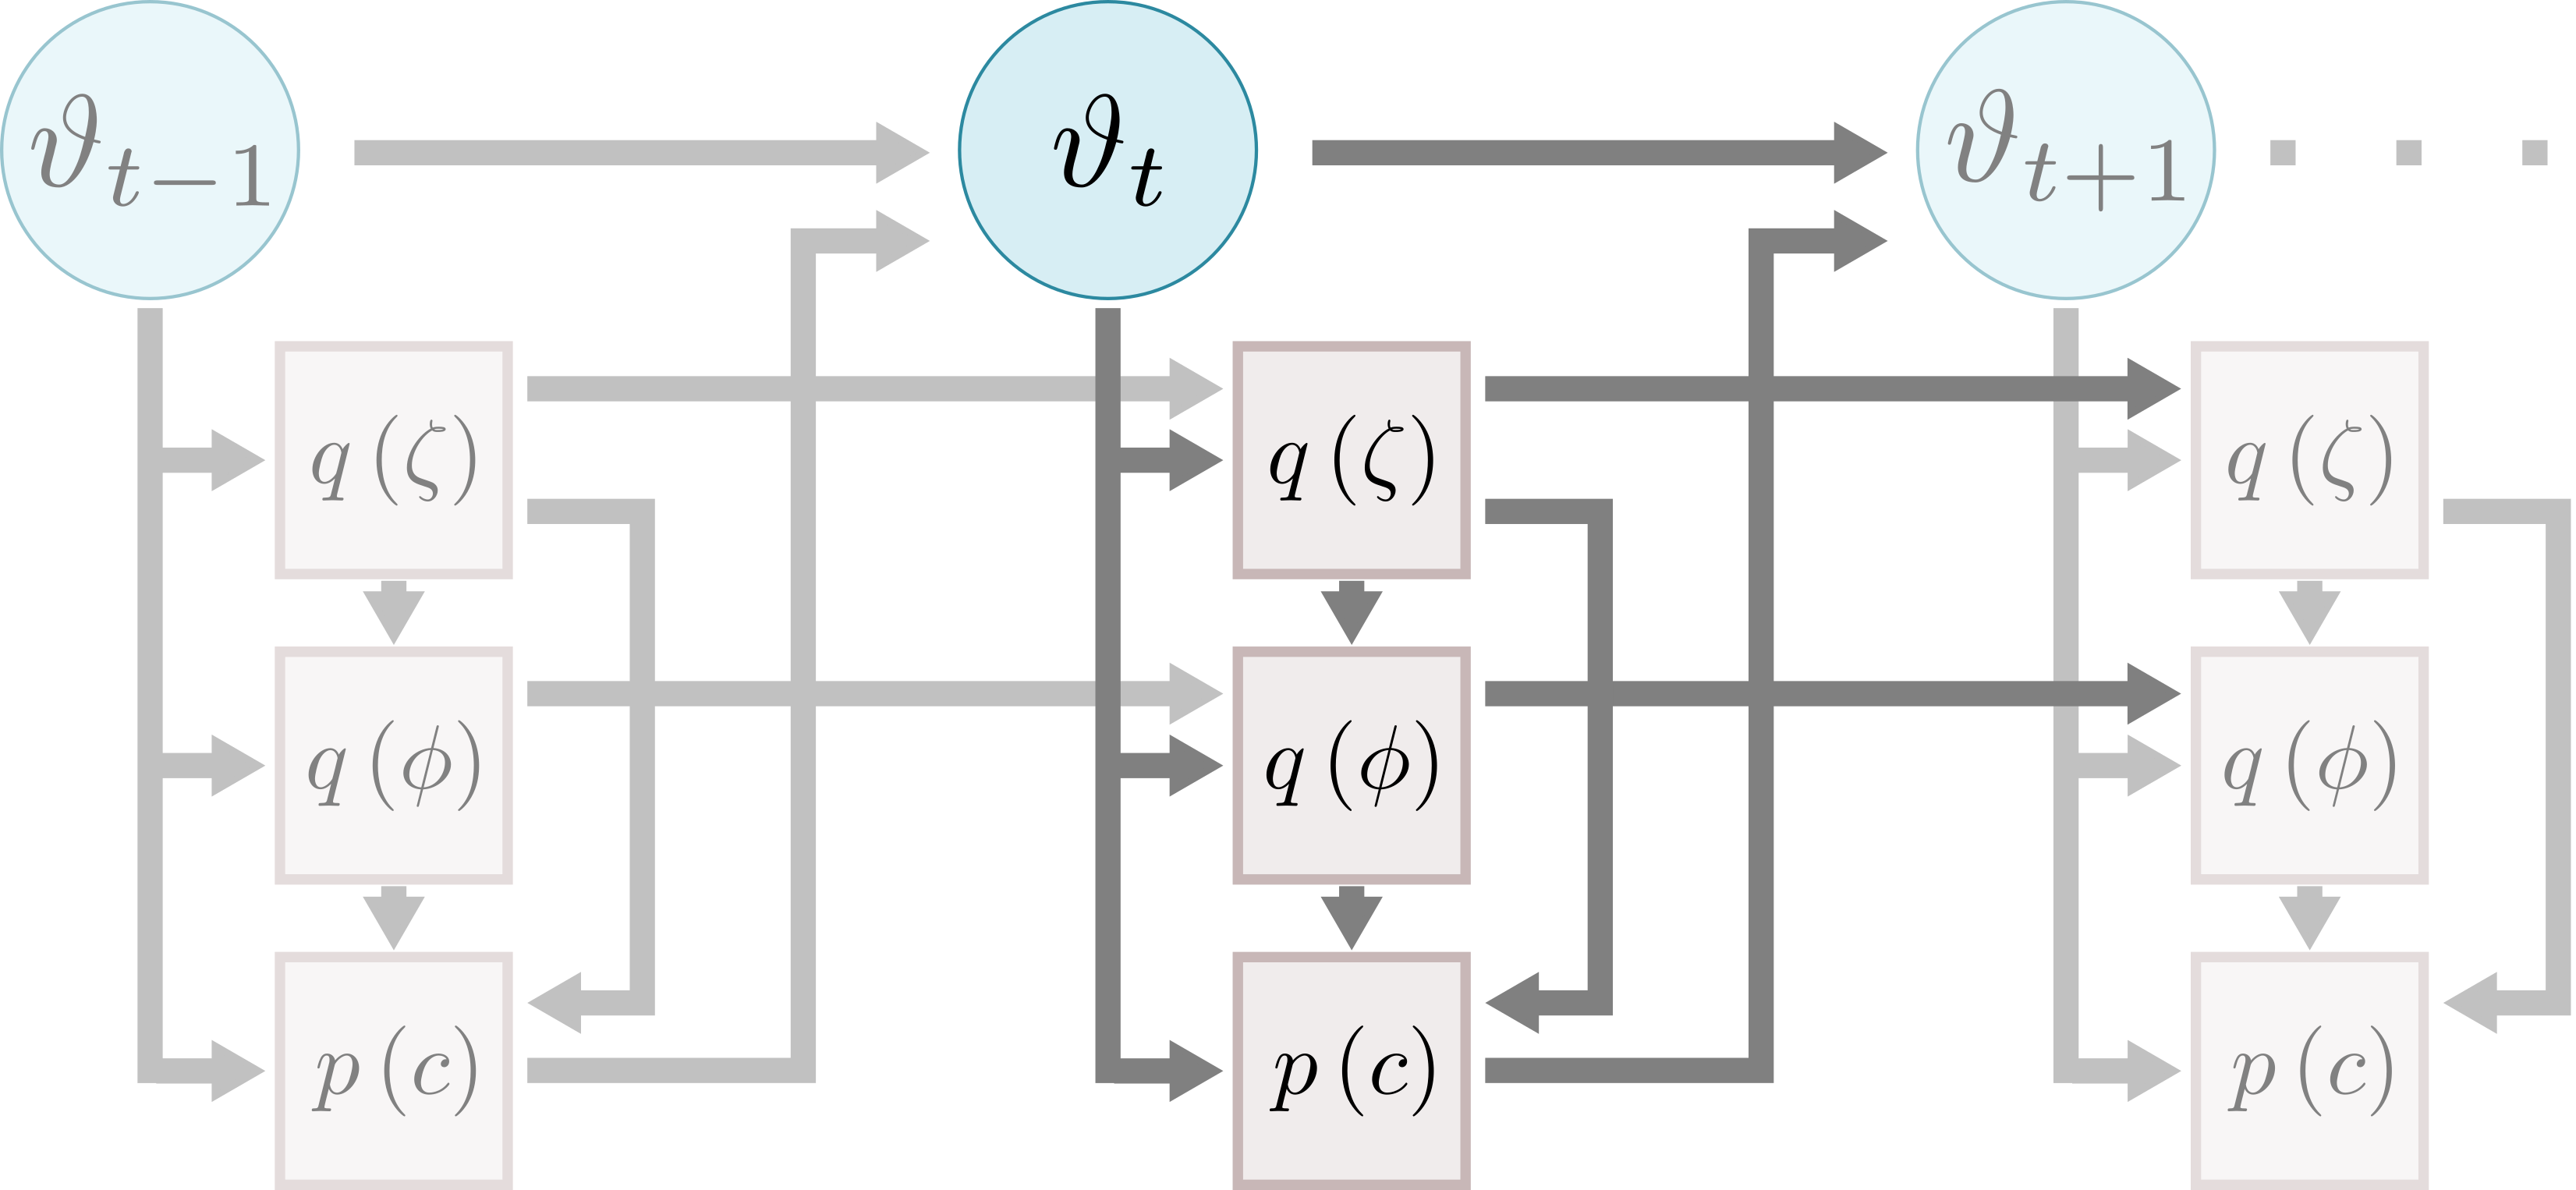
\includegraphics[width=0.7\textwidth]{./figures/figure_1.png}
\caption{Schematic representation of the model and illustrative simulations. (A) Generative model. Clear circles represent the observables, i.e. motor commands $u_t$ and direct observations $y_t$ (e.g. cursor position). The true context $\zeta_t$ is not directly observable, but influences $y_t$. The dark rectangles represent the prior distributions for the inferred adaptation level $x_t$ (Normal-Gamma distribution) and the current context $\zeta_t$ (discrete distribution with known $\pi$; see Methods). At every trial, the context is inferred, then motor adaptation is carried out and finally a motor command is issued; the flow of this process is indicated by the gray arrow in the background, while black arrows show the direction of information flow. (B)\todo{Explain vertical dashes} Simulations obtained with the model in (A), using a simulated experimental setup similar to that by \cite{Davidson_Scaling_2004}. A total of 3x3 experiments were simulated, with low, medium and high levels of both cue uncertainty and observation noise. Each pair of plots represent response/adaptation (top) and context inference $p(ctx)$ (bottom), for one specific level of cue uncertainty and observation noise. In the context inference plot, the y-axis represents the posterior probability of each context $p(\zeta_t = j)$; the black line represents the baseline context (i.e. no adaptation), the green line represents the only adaptation to be learned during the simulated experiment. In the top plot (adaptation), the y-axis is the adaptation to be learned (e.g. the angle in a visuomotor rotation experiment), using the same color scheme (black for baseline). The purple line is the agent's response for the trial. The shaded areas represent the standard deviation around the mean, obtained across 50 simulated participants. The top plots are shown for a single run, for clarity (see main text). All plots share the same x-axis, which represents the trial number.}
\label{fig:model}
\end{figure}
\todo{Remove adaptation plots}
These priors are not mathematically equivalent to those used by \cite{Heald_Contextual_2021}, but the prior samples they produce can be shown to be similar. For more details, see the supplementary materials. \todo{Do this}.

\subsection{Contextual cues and feedback}
The behavioral phenomena which are the focus of this work can be explained as arising from the effects of contextual cues and sensory feedback provided to participants during the experiment. To illustrate these effects in a simple example, we first simulated a generic motor adaptation experiment similar to those performed by \cite{Davidson_Scaling_2004}, in which participants must adapt to a visuomotor rotation of the cursor on a screen in relation to the movement of a pointing device.

The key to an intuitive understanding of the results presented below, is to observe what happens when the presence and reliability of contextual cues is varied, as well as the perceptual noise added to the cursor. In \fref{fig:model}B, a 3x3 grid of results can be seen, where each simulation in this grid is a combination of low, medium or high contextual cue reliability (where low reliability is equivalent to presenting no cues), and low, medium or high perceptual noise.

The first column of \fref{fig:model} shows that, in the presence of reliable contextual cues, context inference is accurate, certain and fast to switch. However, as contextual cues become less reliable, switching between known contexts becomes slower, as seen in the posterior probabilities over contexts at and after trial 20 in the second and third columns. Furthermore, as perceptual noise increases, switching becomes not only slower, but also more uncertain, with individual agents incorrectly missing the switch entirely.

Additionally, the motor responses (shown in purple) can be seen to depend not only on the current estimate of the rotation angle (shown as the green line), but also the uncertainty over the current context. This is most evident in the high cue uncertainty and observation noise panel, in which the response varies substantially from the estimate of the angle (i.e. the purple line deviates from the green line), even when the real context has the highest estimated probability.

As we show below, these effects are at the heart of the behavioral phenomena observed in the experiments by \cite{Kim_Neural_2015}, \cite{Oh_Minimizing_2019}, \cite{Davidson_Scaling_2004}, and \cite{Vaswani_Decay_2013}, which we directly simulate in this work, alongside others that we discuss in the Discussion section.



\subsection{Experimental results}
In this section, we present experimentally-observed phenomena in three sections, and show that the dynamics of context inference provide a unifying explanation for all of them. In the first section, we discuss switches between contexts, and how slow context inference affects these switches. In the second section, we focus on interference between learned adaptations. Finally, in the third section we discuss context inference during error-clamp trials, and its effect on behavior. For each of the three sections, we selected one or two studies which are representative of the phenomenon being discussed.

For clarity, we first introduce necessary terminology that is typically used in experimental studies. As an example, we will use a typical motor adaptation task in which participants have to make reaching movements while holding the handle of a mechanical arm that exerts a curl force on the participant's hand. Depending on the trial, the mechanical arm might exert a curl force in a clockwise or counter-clockwise direction, or no force at all. Let us define the baseline context O as that in which the mechanical arm exerts no force. Contexts A and B can be defined as those with clockwise or counter-clockwise, respectively. Abusing notation, a usual statement is that $B = (-A)$, as the forces have the same magnitude but point in opposite directions. Similarly, one can define context A/2, with the same direction of adaptation as A, but half the magnitude. Finally, many experiments include a block of error-clamp trials at the end of the experiment, in which the mechanical arm forces the participant to make straight-line movements; we represent these with the letter E.

With this terminology, a typical experiment \cite[e.g.][]{Ethier_Spontaneous_2008} would have a block structure of O-A-B-E, or O-A-(-A)-E, which means that the participant goes through a block of trials with no external force applied (O), a number of trials with a clockwise curl force (A), a block with counter-clockwise forces (B), and finally a block with error-clamp trials (E). With repeated contexts \citep[e.g.][]{Oh_Minimizing_2019}, an experiment can be described as $O_1$-$A_1$-$O_2$-\ldots .

\subsubsection{Savings and slow/fast switching}
The term 'savings' refer to the ability to remember a previously-learned adaptation and apply it without having to re-learn it. Savings is almost universally observed in humans \citep{Brashers-Krug_Consolidation_1996,Shadmehr_Functional_1997,Medina_Mechanism_2001,Smith_Interacting_2006,Zarahn_Explaining_2008}. In an O-A-O-A experiment, for example, savings would express themselves in the second A block in the form of a much higher adaptation rate than that observed during the first A block. The related concept of quick de-adaptation occurs in A-O transitions, where participants switch back to baseline without having to re-learn it.

In this section, we discuss savings and de-adaptation in terms of switching between contexts. We show that through context inference and how it is affected by contextual cues and observation noise, savings are not immediate, but a relatively fast process that reflects context inference.

To show this, we examined multiple experimental studies in which savings are observed. We categorized these studies based on the amount of contextual information made available to participants: In some experiments \citep[e.g.][]{Kim_Neural_2015,Lee_Dual_2009}, the context is clearly revealed to the participant using sensory cues. We call these cued-context experiments. In other experiments, partial information is available to participants \citep[e.g.][]{Davidson_Scaling_2004,Zarahn_Explaining_2008} in the form of large prediction errors, partial contextual information or reward prediction errors; we refer to these as partially-cued experiments.

We selected three representative experiments from two studies \citep{Kim_Neural_2015,Oh_Minimizing_2019} which differ in the amount of contextual information available to participants. \cite{Kim_Neural_2015} performed a cued-context visuomotor rotation experiment with three contexts with different rotation: no rotation, 40 degrees and -40 degrees. Participants performed shooting movements in blocks of trials with the same rotation. Importantly, a colored light identified the current context, making this a cued-context experiment. Consistent with the context-inference account, the authors found that switching was immediate and accurate.

In \fref{fig:oh-2019}A we show the results of simulations with the model using the parameters of the task, as well as the experimental results from \cite{Kim_Neural_2015}. The correspondence between simulations and experimental results can be seen in the switches between contexts in the center panel, i.e. when the solid gray line (representing the true context) switches between 40, 0 and -40; in both panels (second and third), the thick black line, representing the agent's adaptation, quickly follows these switches.

\begin{figure}
\centering
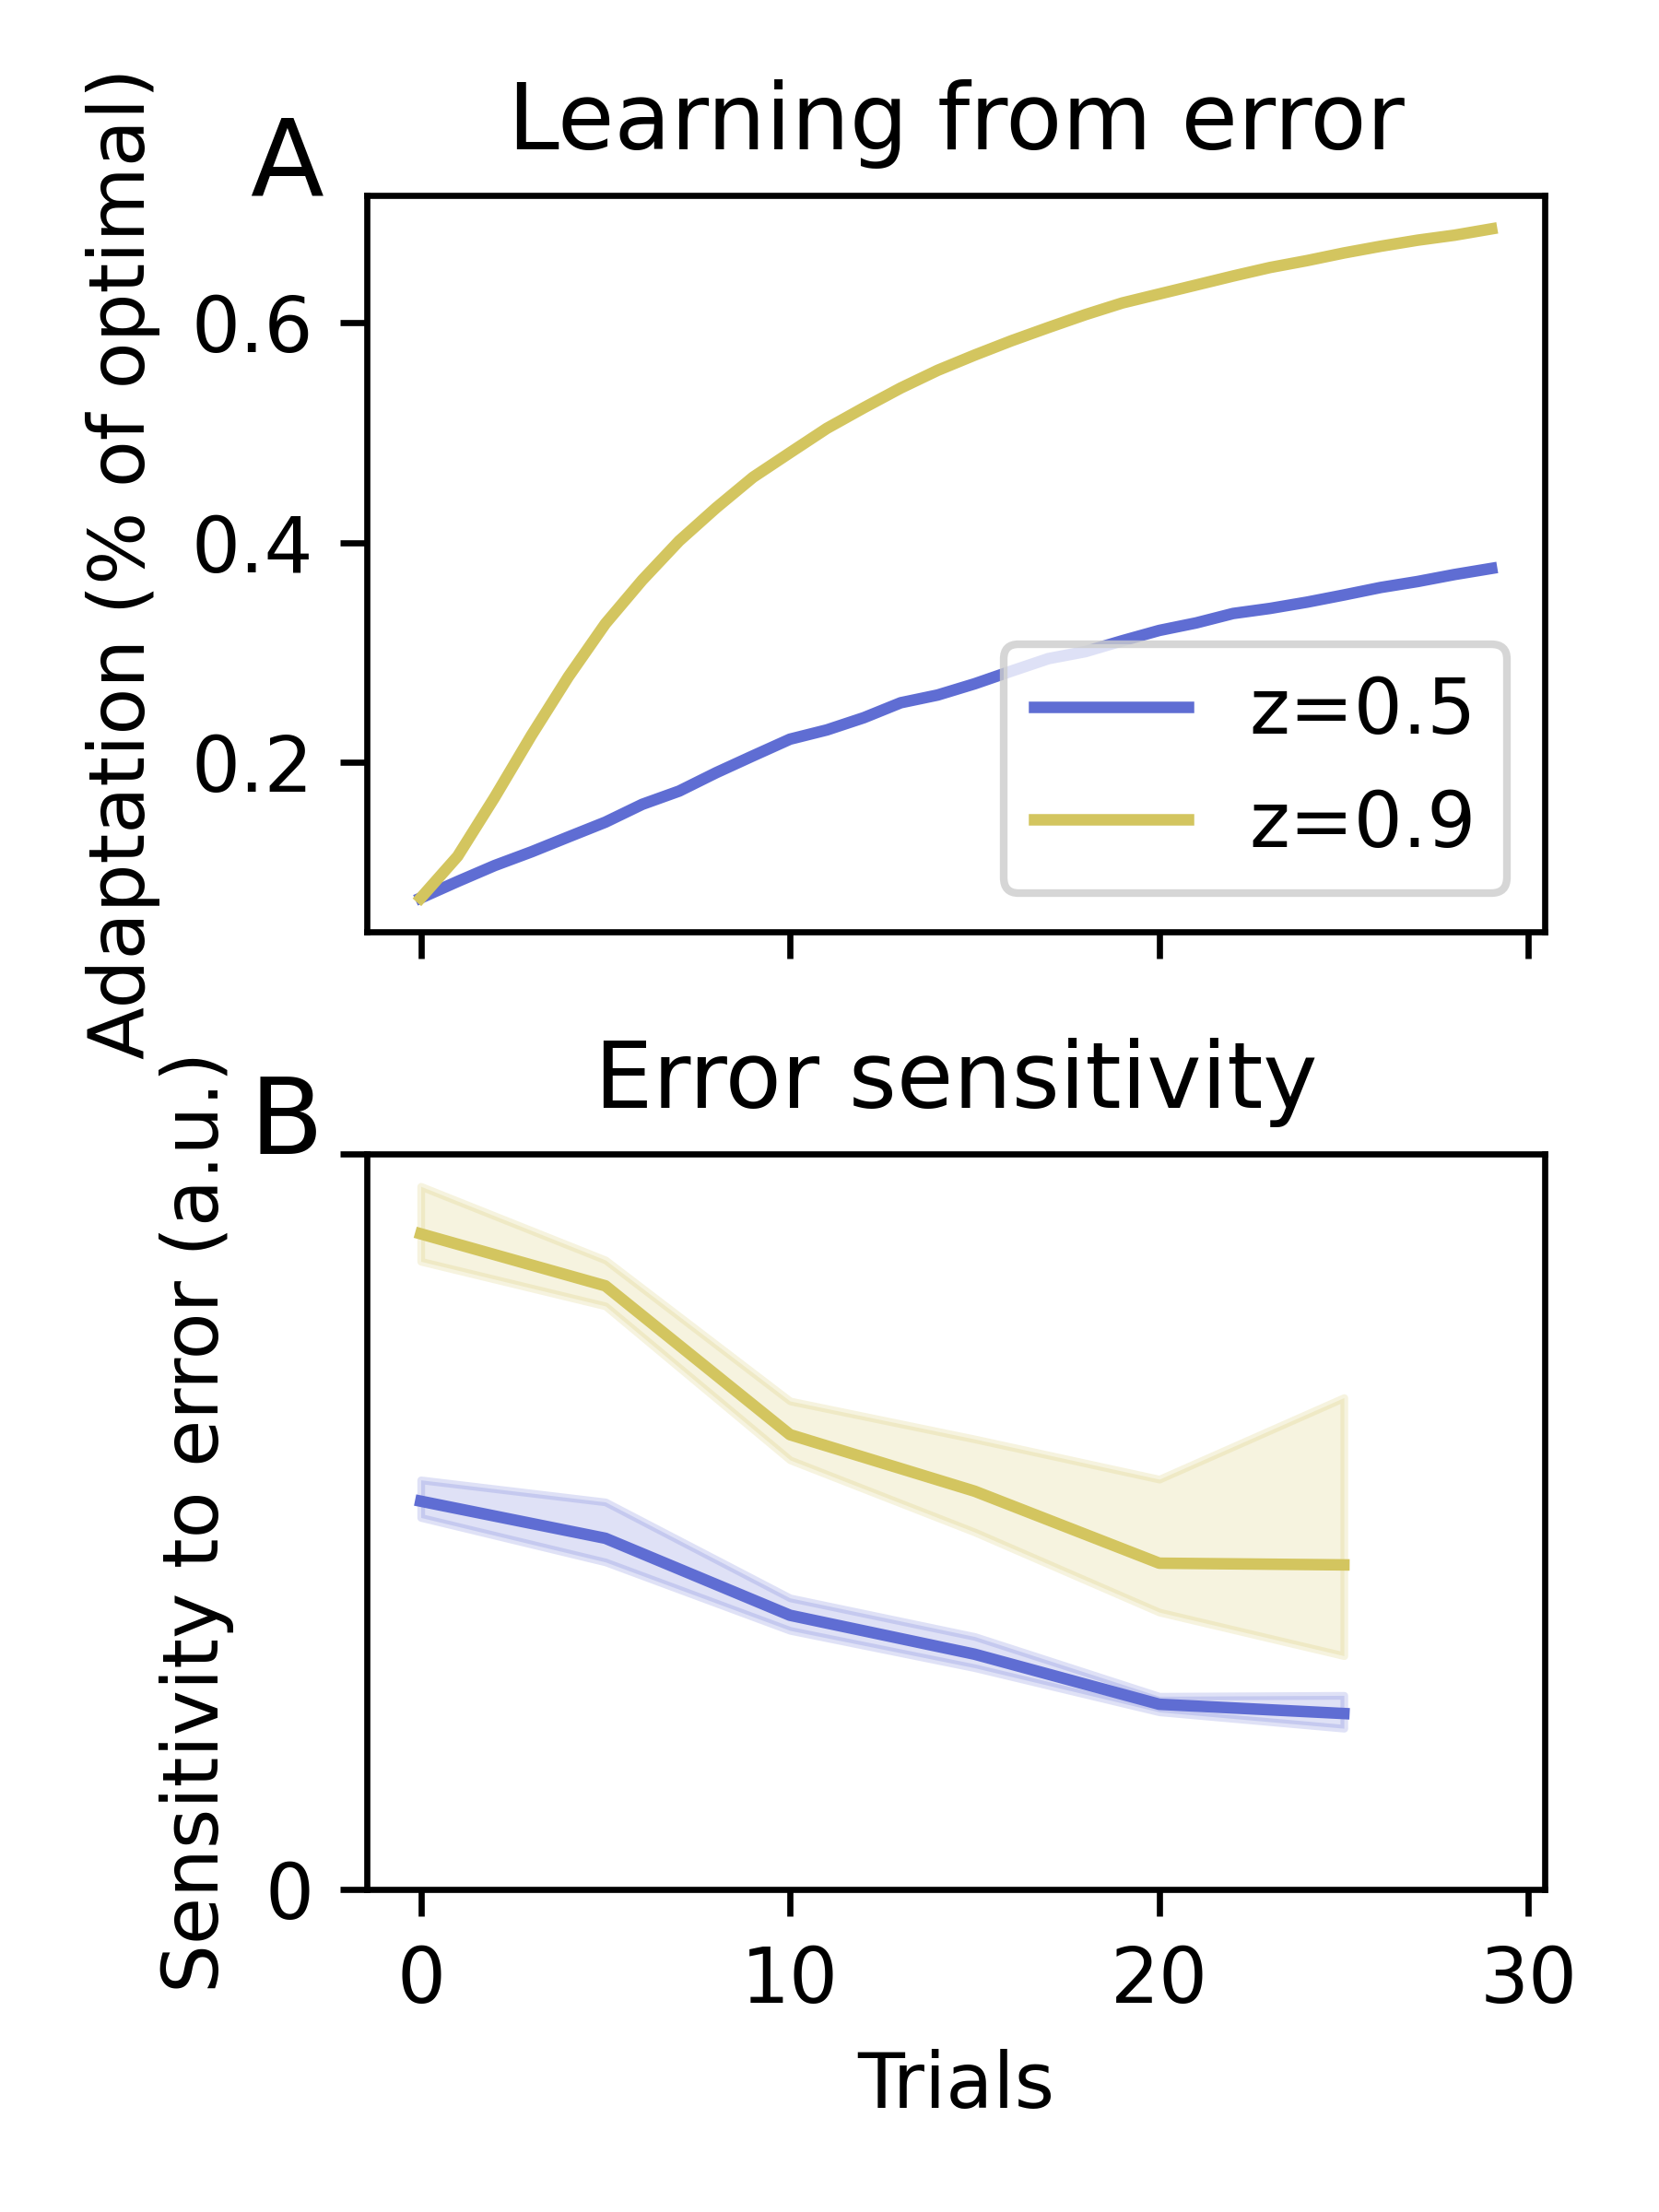
\includegraphics{./figures/figure_2.png}
\caption{Savings and de-adaptation. Data from our simulations (first and second columns) compared to data adapted from figure 2A by \cite{Kim_Neural_2015} and figure 4A from \cite{Oh_Minimizing_2019} (last column). Experimental data was, in all three experiments, averaged across all participants; in our simulations, a single simulation is shown. In the first column, the simulated context over inference is represented by the posterior probabilities over all available contexts. Each color (black, blue, green) represents a different context, with black always representing the baseline (i.e. no adaptation). Vertical, dashed lines represent switches in the real context. In the second and third columns, the black line represents the adaptation (i.e. response) displayed by the agent as a function of trial number. The thin gray lines represent the optimal adaptation, i.e. the size of the true visuomotor rotation during the task. In all panels, the x-axis represents trial number, from 0 to 300. (A) Experiment by \cite{Kim_Neural_2015} with two visuomotor rotations (-40 and 40 degrees), in addition to baseline, with all possible transitions between A, (-A) and O. Participants must adapt to the rotations during shooting movements, and the participant's response can be understood as the rotation of the participants' shooting movements to compensate for the task's rotation. For clarity, both experimental and simulated results are shown only up to trial 300, of the original 600. (B) An experiment by \cite{Oh_Minimizing_2019} similar to (A), but the contexts were not cued and only one context, with an adaptation of 20 degrees, is introduced. O-A and A-O transitions (i.e. adaptation and de-adaptation) can be observed. Blue and black lines are as in A. (C) Same experiment as (B) but with a 10 degree adaptation.}
\label{fig:oh-2019}
\end{figure}

Critically, in \fref{fig:oh-2019}A it can be seen for the first four context switches (until about trial 250) that participants had not yet completely adapted to the rotation, as evidenced by their responses not being on par with the true rotation angle. This undershooting of responses (i.e. not doing the 40 degree rotation) happens despite participants being able to immediately and with high certainty identify the true context, as shown in the first-column panel. These results are similar to those shown by \cite{Imamizu_Explicit_2007}, where sensory cues of varying reliability effected immediate or slow contextual switches.

To expand on these results, we now turn to feedback and its effects on switching behavior. \cite{Oh_Minimizing_2019} performed two partially-cued experiments with a visual rotation of 20 and 10 degrees, respectively. The results of their experiments can be seen in \fref{fig:oh-2019}B and \ref{fig:oh-2019}C, alongside simulations with the COIN model. Participants in the first experiment (\fref{fig:oh-2019}B) first learned the adaptation in $A$. In subsequent $A - O$ transitions, participants showed immediate switching (with a one-trial lag) between A and O (both ways), which can be seen in their responses (black line in the last two columns of \fref{fig:oh-2019}B) closely following the switches in the black line (true rotation). In the second experiment (\fref{fig:oh-2019}C), switching happens more slowly, with adaptation lagging behind the switches in the real context, and slowly catching up. As can be seen in the left panels in \fref{fig:oh-2019}B and \ref{fig:oh-2019}C, the same model parametrization produces fast, accurate switches when the adaptation is large (B), and slow, noisy switches when it is low (C). This difference is explained in our simulations in terms of the size of the adaptation in relation to observation noise: as the adaptation is smaller (10 degrees), it becomes more difficult to distinguish errors made by incorrectly inferring the context from the noise due to trial-to-trial variation in motor output. Because of this, the model requires more evidence (i.e. more trials) to infer a switch in contexts.

Note that the results from our simulations from \cite{Oh_Minimizing_2019} and from \cite{Kim_Neural_2015} include both savings (O-A transitions) and de-adaptation (A-O transitions), both of which display the same characteristics and are explained by the same mechanism.

\subsubsection{Uncertainty over contexts affects action selection}
As with learning, action selection is affected by context inference. If the identity of the current context is known, the forward model for this context is used to select the current action. However, if uncertainty over the context exists, the selected action is influenced by all the possible contexts, with a weight directly related to how likely each one of those contexts is (see \eref{eqn:dist-comm}).

Experimental evidence supporting this view can be found in experiments with context switching. For example, \cite{Davidson_Scaling_2004} reported a curl-force experiment in which participants had to switch from 3A to A in one group, with a block sequence A-3A-A-3A, and from -A to A in another group, with a block sequence A-(-A)-A-(-A). After A and 3A (or -A in the other group) had been learned in the first two blocks, the authors found that the switch from 3A to A was faster than that from -A to A. The authors interpreted this as evidence that switching between adaptations happens more quickly if it is in the same direction as the current adaptation (e.g. both counter-clockwise), and more slowly if they are in the opposite direction (e.g. clockwise to counter-clockwise).

Under the COIN model, the asymmetry is caused by the existence of the baseline context, which has a non-zero probability $p(\zeta_O | s_t ...)$. When a new block of trials starts (e.g. in the transition from 3A to A), a switch is inferred by the model (given feedback after the first trial) and $\zeta_O$ becomes more likely (given that $\zeta_{3A}$ has been ruled out). Therefore, in these first trials, action selection has a component guided by the baseline model, in which no extra compensatory force is applied, effectively ``pulling'' adaptation towards zero (no compensatory force). In the first group, this initial pull towards zero accelerates the transition towards A because $3A > A > 0$, but in the second group, it slows down the switch because $A > 0 > -A$.

We simulated data with the model fitting the experimental structure in \cite{Davidson_Scaling_2004}. We show the results in \fref{fig:davidson-2004}A, alongside the experimental results from \cite{Davidson_Scaling_2004}. It can be seen that the agent exposed to the -A context shifts back to A more slowly than the one exposed to 3A, qualitatively reproducing the data from \cite{Davidson_Scaling_2004}.

\begin{figure}
\centering
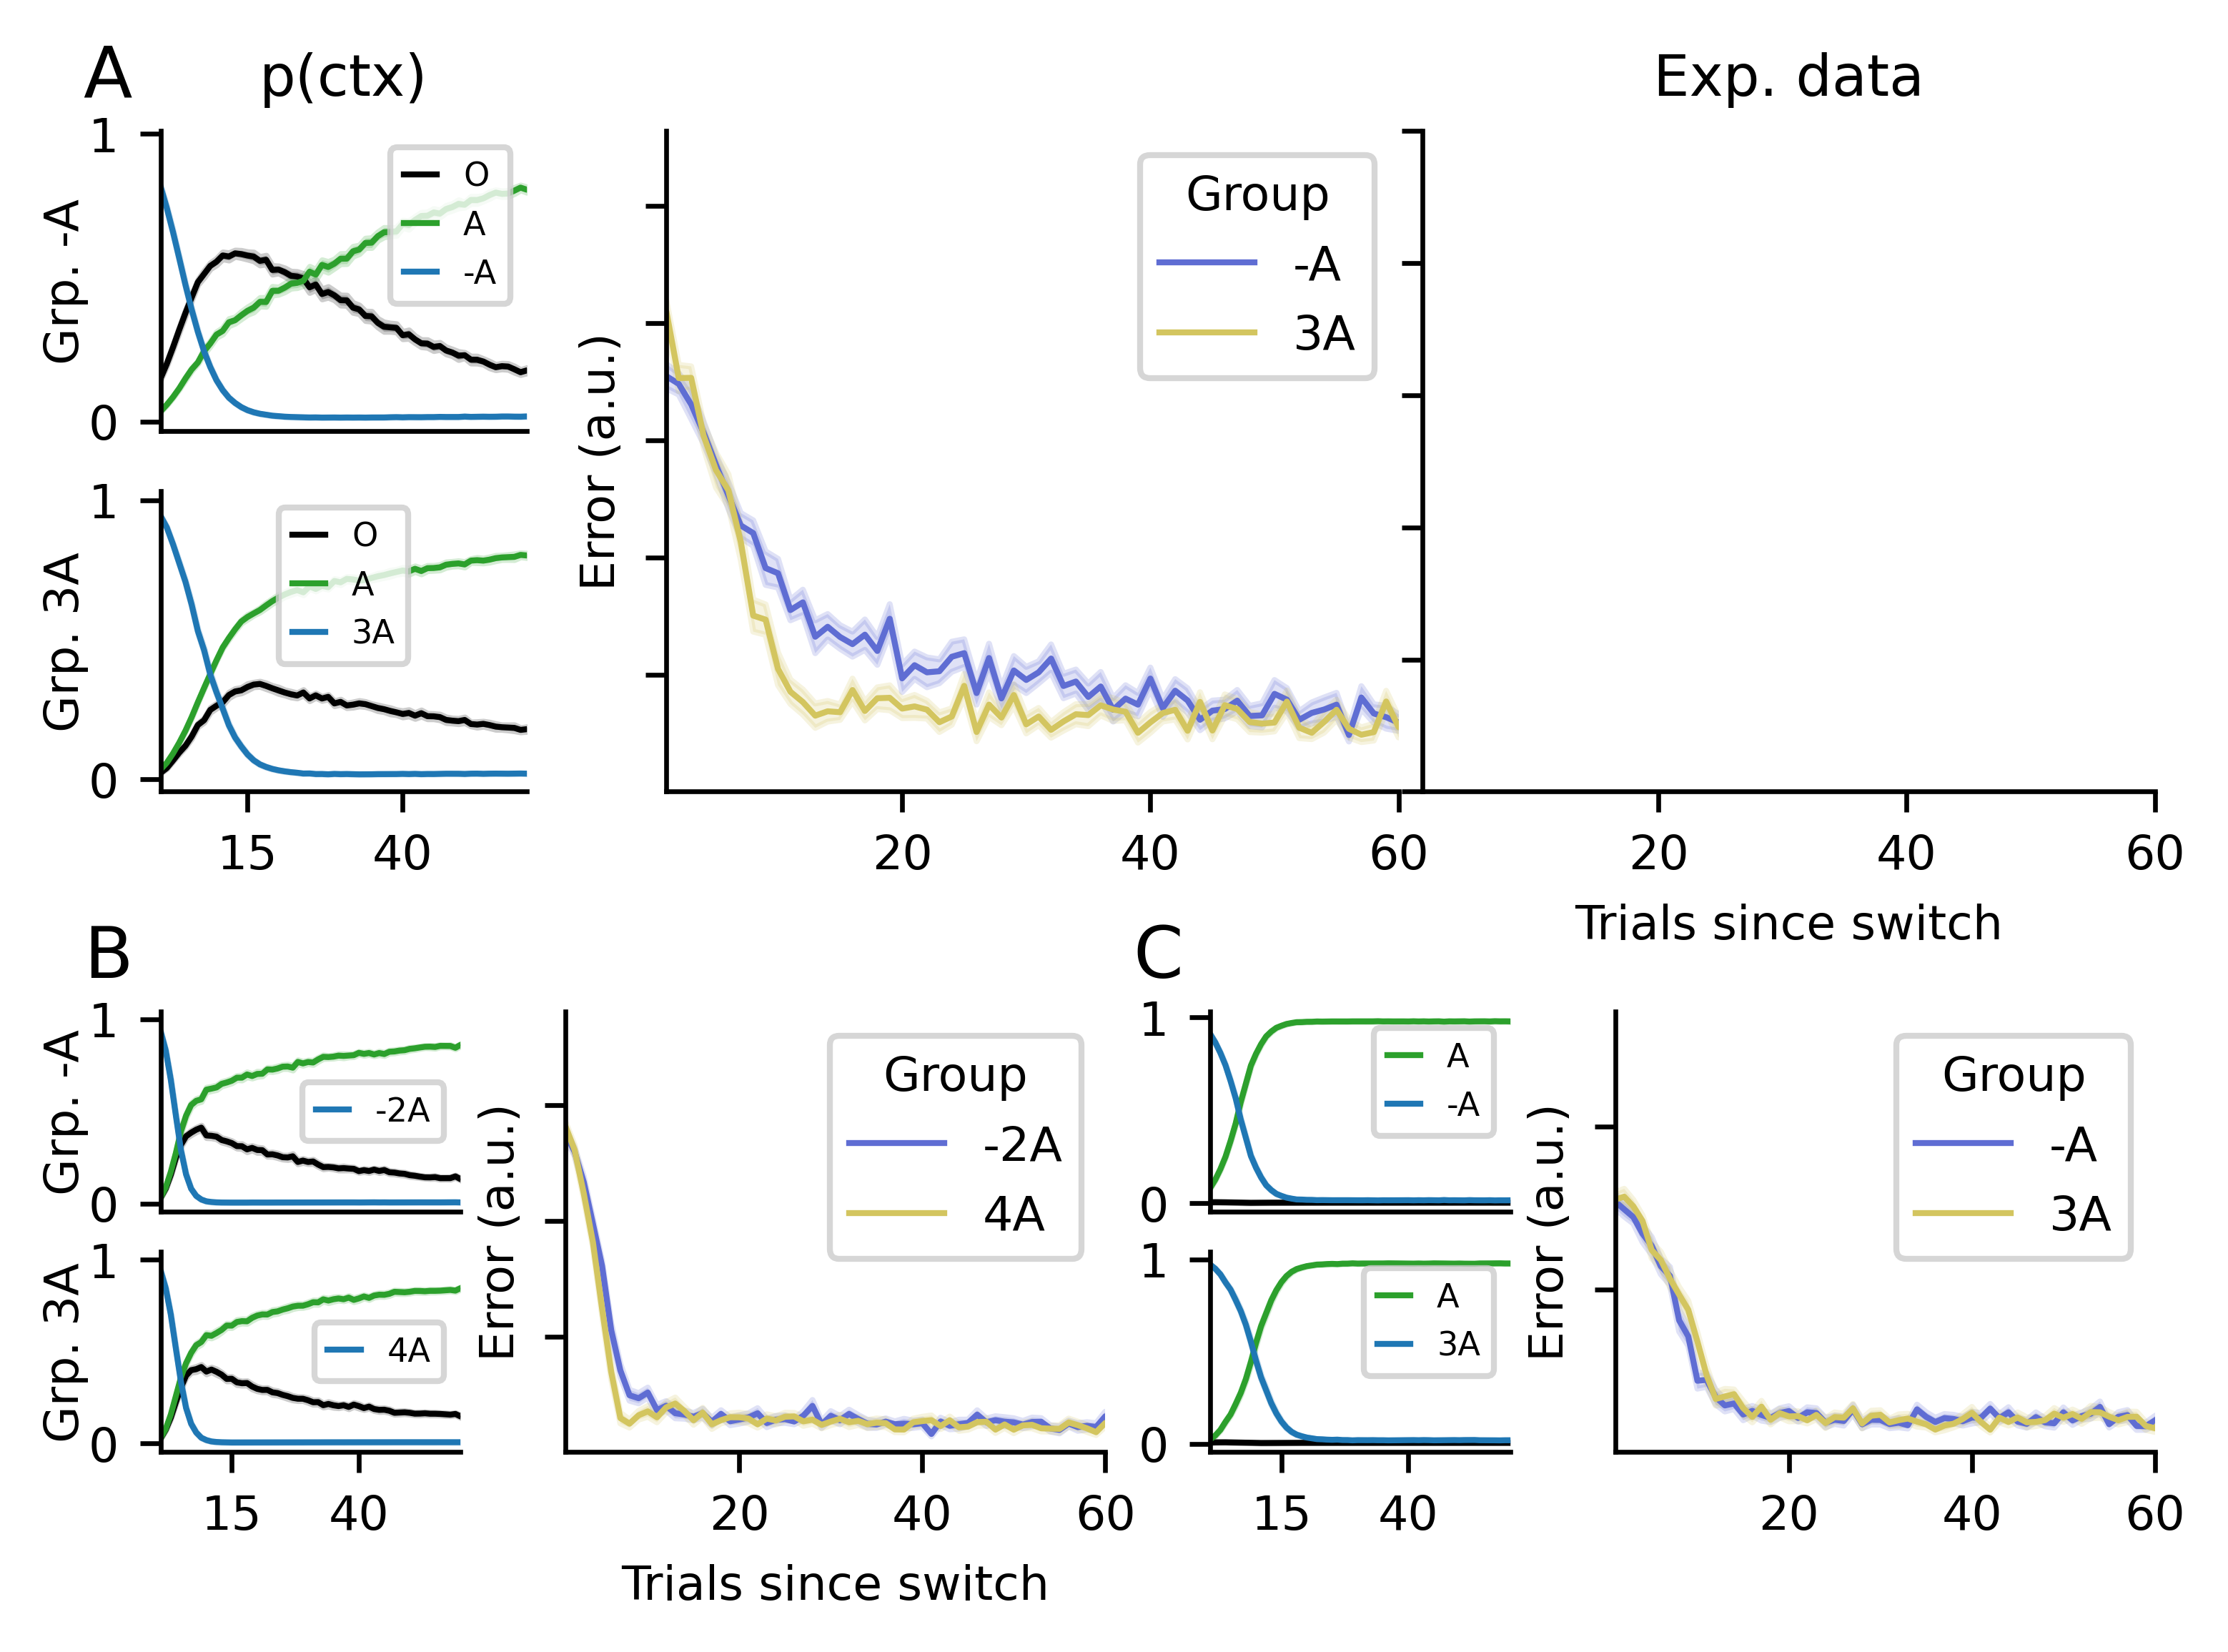
\includegraphics{./figures/figure_3.png}
\caption{Motor error when switching back to a previously-learned adaptation. (A) Experimental results from \cite{Davidson_Scaling_2004} and simulations with the COIN model are shown. In the first column, each panel represents context inference for one group of participants (top: group A; bottom: group 3A), with each line representing the posterior probability of a context (black for the baseline O). The second column represents the error made by our simulated agent after returning to the previously-learned context, with blue and yellow representing groups -A and 3A, respectively. The last panel represents the same data, from the \cite{Davidson_Scaling_2004} experiment. All panels share the x-axis, representing the number of trials elapsed since the switch to the new context. All simulations were executed eight times per group, following the number of participants in the experiments; shaded areas represent the standard deviation across these eight simulations. (B) Simulated results for an experiment similar to \cite{Davidson_Scaling_2004}, but changing the contexts seen by the two groups from -A to -2A for the first group, and from 3A to 4A for the second group. The panels follow the same structure as (A), without the last panel for experimental results. (C) Simulations for an experiment in which the baseline context has been removed altogether.}
\label{fig:davidson-2004}
\end{figure}

To confirm our hypothesis, we simulated variants of the experiments in which the COIN model predicts that the difference between groups disappears. First, in \fref{fig:davidson-2004}B, we simulated an experiment in which the contexts have more extreme adaptations, making them more different from baseline than in the \cite{Davidson_Scaling_2004} experiments. To do this, one group adapts in a $O-A-(-2A)$ paradigm, while the other group adapts in a $0-A-4A$ paradigm. As in the original experiment, the second contexts ($-2A$ for one group, $4A$ for the other) are equally spaced from the first context. However, given the larger distance from baseline, the baseline context has a much lower attribution when the switch occurs compared to the original experiment. This change makes both simulated groups infer the correct context almost equally quickly, making the difference between their errors much smaller compared to the original experiment. Furthermore, we simulated an experiment with an identical structure to that of \cite{Davidson_Scaling_2004}, but eliminated the baseline context from the agent. The results can be seen in \fref{fig:davidson-2004}C, where the switches between contexts are made identically by the two groups. We discuss possible implementations of such an experiment in the Discussion section, alongside with other predictions made by the model. \todo{Promises, promises} 

\subsubsection{Action selection in error-clamp blocks}
During error-clamp blocks at the end of block sequences, participants' behavior can be divided in two phases: (1) Spontaneous recovery, during which participants' behavior is consistent with a previously-encountered context (e.g. in an O-A-E experiment, consistent with A); this phase, when present, is seen during the early trials of the E block. (2) A slow return to baseline, which can last as long as hundreds of trials \citep{Brennan_Decay_2015}. However, the direction of the spontaneous recovery, its duration, the delay before it is observed, the speed of the return to baseline and the final asymptote of the adaptation vary greatly depending on the experiment \citep{Brennan_Decay_2015,Vaswani_Decay_2013,Smith_Interacting_2006,Shmuelof_Overcoming_2012}.

In this section, we show how context inference can explain these different parameters of behavior by changing the way contextual cues mislead participants' context inference, which in turn influences action selection.

This can be seen for example for \cite{Vaswani_Decay_2013}, who studied in detail human behavior during an error-clamp block in a shooting movement paradigm with a mechanical arm. The authors found that during an E block at the end of each experiment, there was a lag of a few trials (depending on participant) before their motor behavior changed from that of the previous block. After that, the exerted force slowly dropped towards zero throughout tens of trials, but never reaching values around zero. Participants were divided into four groups, each of which going through a different block sequence: (1) A-E, (2) O-A-E, (3) (-A/2)-A-E, and (4) (-A)-E. No pauses were made during the experiment nor were there any contextual cues, so transitions between blocks were not signaled to participants. However, because context inference integrates information from different sources, many experiments in which no intentional, overt contextual cues are available indeed contain contextual information that the participant can use to infer the context. For example, proprioceptive signals  provide contextual information \citep{Dizio_Motor_1995,Shadmehr_Adaptive_1994}. The sudden appearance of motor errors can itself be a cue for contextual change \citep{Herzfeld_memory_2014} and even a pause between two trials could suggest a change in context \citep{Ethier_Spontaneous_2008}.

In \fref{fig:vaswani-2013}A, we show data simulated with the COIN model, following the parameters of the experiment by \cite{Vaswani_Decay_2013}, and in \fref{fig:vaswani-2013}B we show the experimental plots adapted from \cite{Vaswani_Decay_2013}. The displayed adaptation is shown during the E trials for the three experimental groups in the experiment. It can be seen that group 1.3 (i.e. the participants who had learned in the -A/2 context in addition to A) more quickly recognized a change in context and lowers the force applied on the mechanical handle, as can be seen in the experimental data.

\begin{figure}
\centering
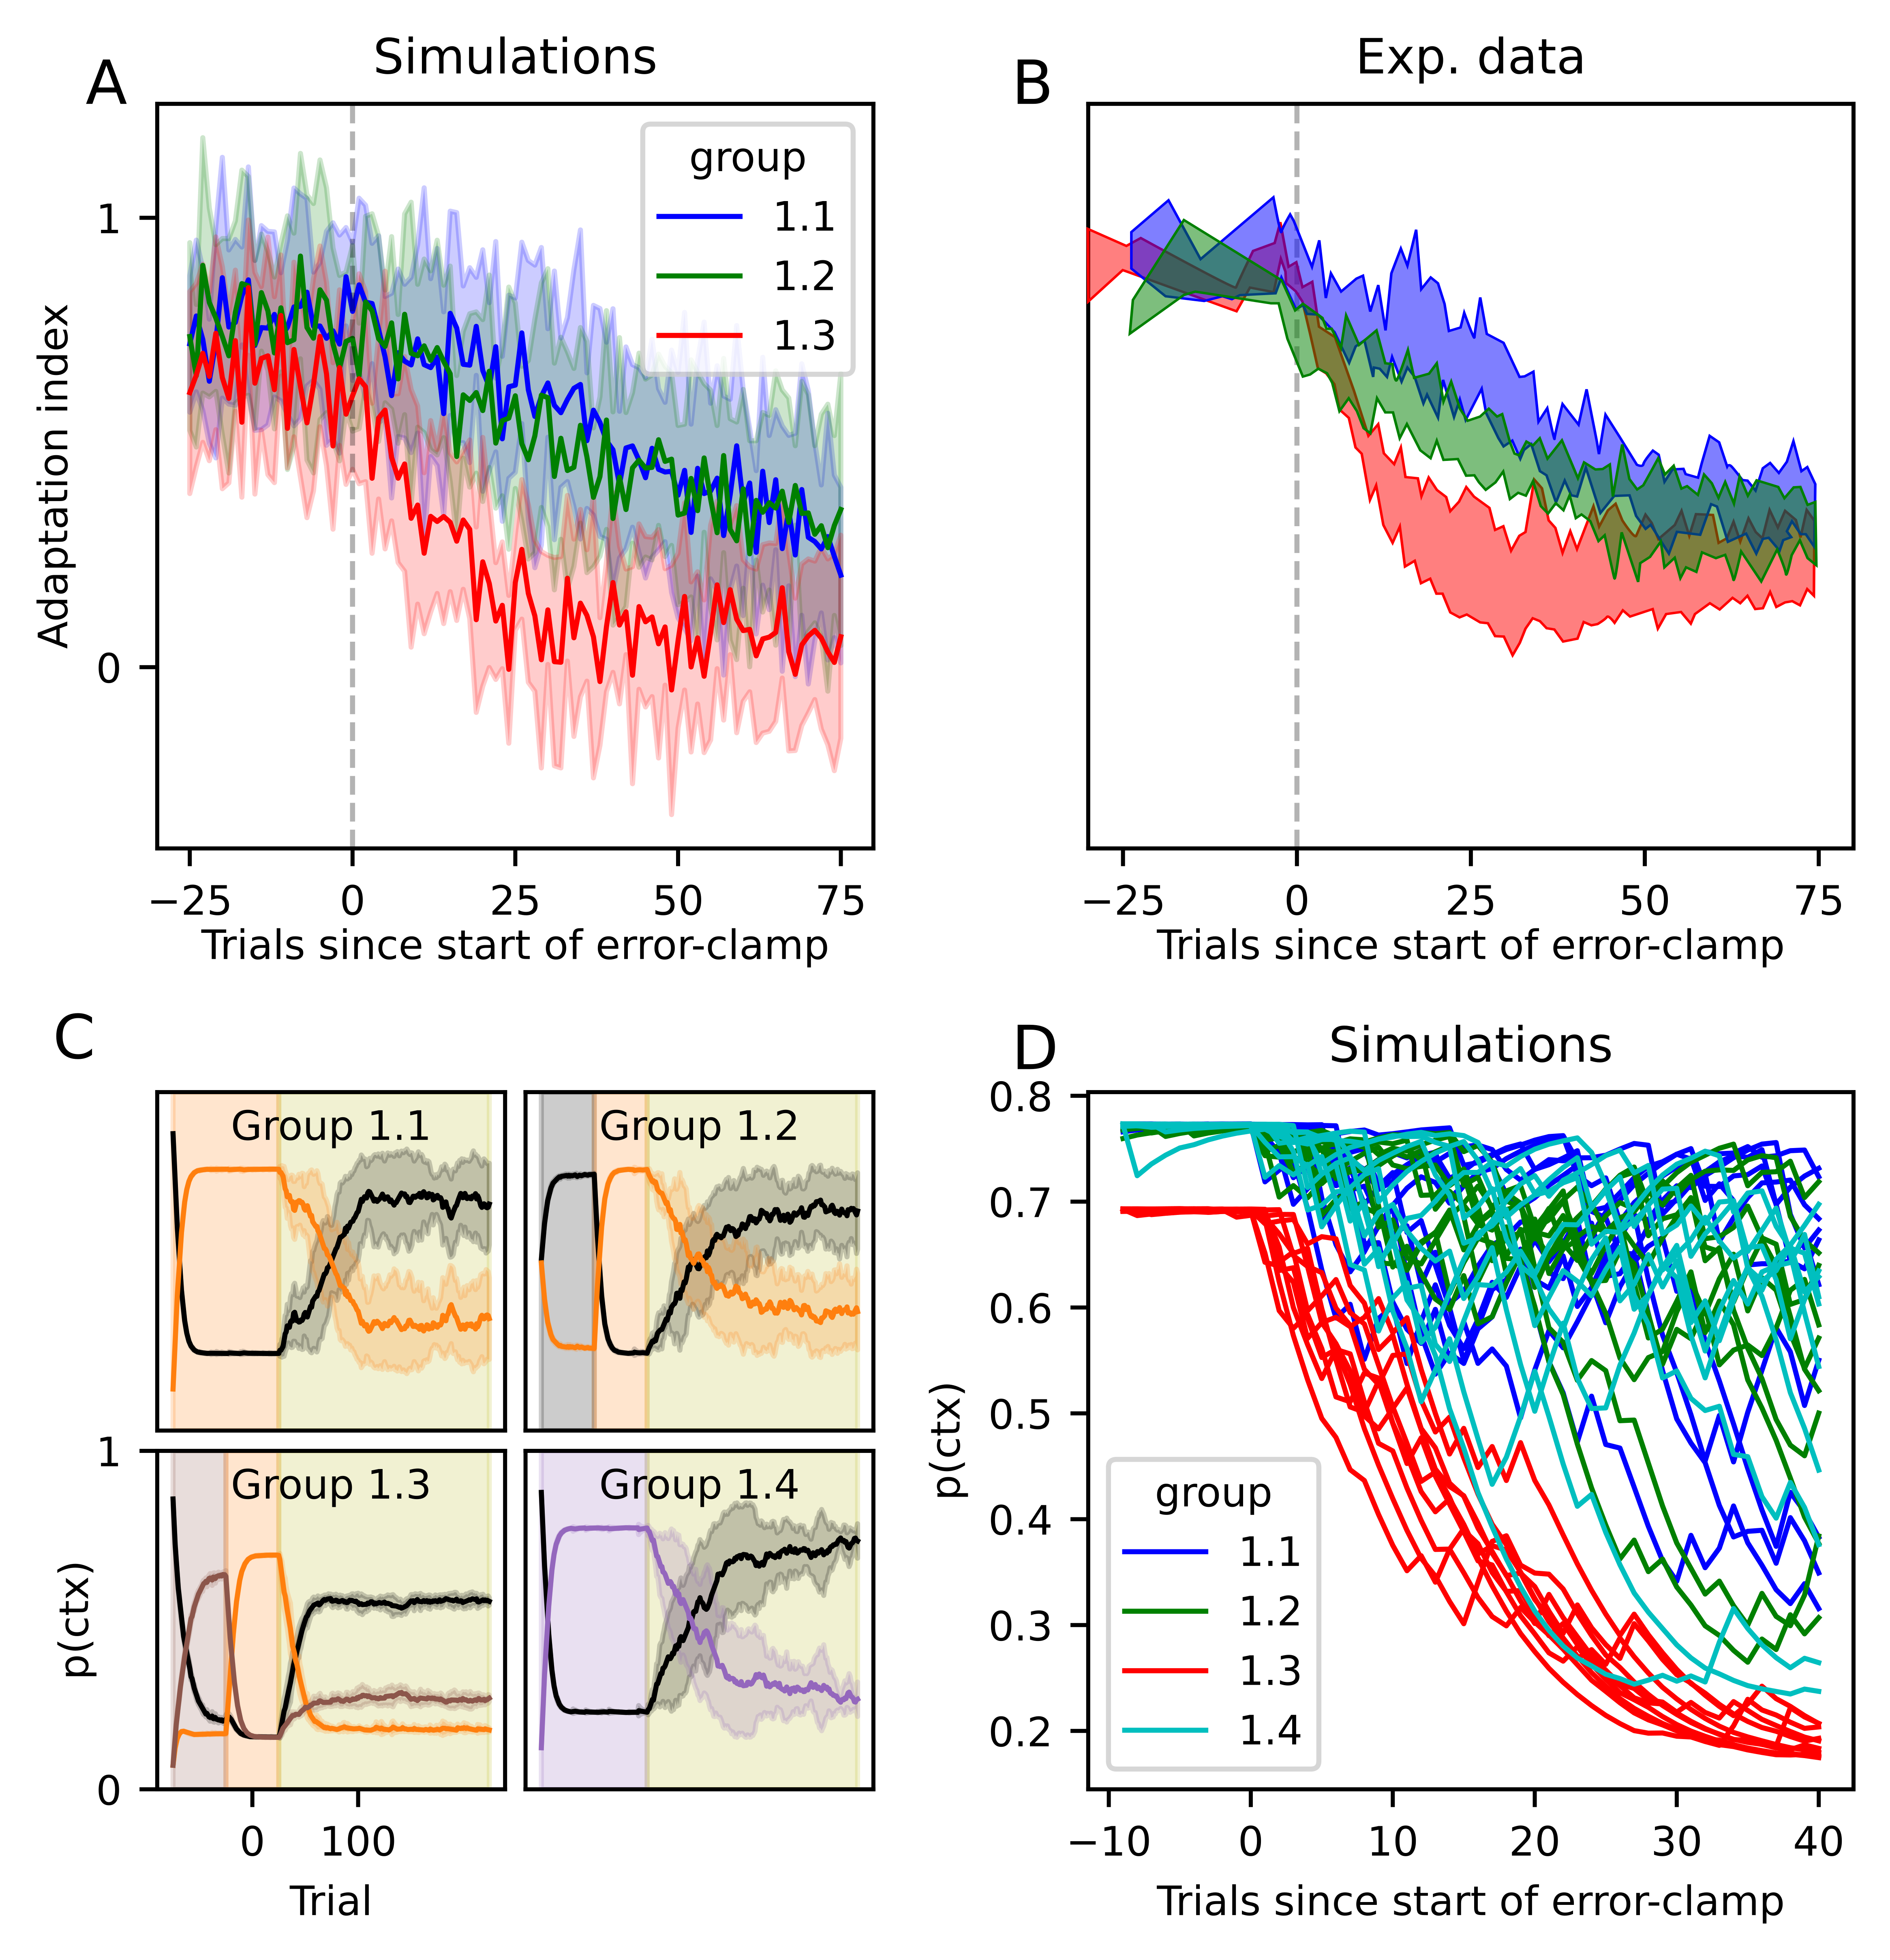
\includegraphics[width=\textwidth]{./figures/figure_4.png}
\caption{Adaptation during error clamp trials. (A) Simulated adaptation during the error-clamp trials for the three groups of participants in \cite{Vaswani_Decay_2013}, using the same colors. The groups differ in the sequence of adaptations: 1.1 performed an A-E sequence; 1.2, O-A-E; 1.3, (-A/2)-A-E; and 1.4, (-A)-E. Following \cite{Vaswani_Decay_2013}, group 1.4 is not shown in A and B, as their behavior is identical to group 1.1. The solid line is the average across 10 runs (i.e. a group of 10 simulated participants) and the shaded area represents the standard deviation. The vertical dashed line is the start of the error-clamp trials. (B) Corresponding experimental data adapted from figure 2C by \cite{Vaswani_Decay_2013}. (C) Simulations: Inference over the current context, where contexts are color coded: black for baseline, orange for the counter-clockwise force, purple for the clockwise force and brown for counter-clockwise force with half strength. The lines represent the posterior probability of each context in every trial, while the background color represents the true context. An olive-colored background represents error-clamp trials. As in (A), solid lines represent the average across all runs and shaded areas represent the standard deviation. (D) Simulations: Visualization of the lag before a change in context is detected by the agent during the E trials. Each line represents one run (10 runs per group).}
\label{fig:vaswani-2013}
\end{figure}

In \fref{fig:vaswani-2013}C, the inference over context is shown for each group separately. Context inference works reliably until the error-clamp trials start, which do not correspond to any of the known contexts. This causes the agent to infer the combination of some of the known contexts that best fits the observations. Depending on the contexts previously learned by the agent: groups 1.1 and 1.4 display the same behavior, where the previous context (A and -A, respectively) slowly dwindles. These agents will slowly lower the force applied. In contrast, group 1.3 has learned the additional -A/2 context, which has a non-zero posterior probability during E trials, pushing the agent's adaptation force more quickly towards zero. Group 1.2 behaves similarly to 1.1, with the exception that the baseline context, which was recently seen, plays a bigger role during E trials, making the agent reduce its force during E trials slightly more quickly than groups 1.1 and 1.4. \todo{Danger! Danger! A keen observer might point out that the model might want to learn a new context, as COIN does. What to do? What to do?}

Context inference also explains the variability in the lag before adaptation starts to drop to zero after the E block starts. In the model, this lag is due to a period in which context inference has not ``caught on'' to the change of context; during this period, behavior remains consistent with that of the previously-observed block, as can be seen in the experimental data as well. To show this, we show in \fref{fig:vaswani-2013}D the drop in the inferred probability of the previous context for each simulated run (one line per run, 10 runs per group, all groups). The start and speed of the drop depend on the run (i.e. the participant), reproducing the different lags observed in experimental data.

\section{Discussion}
We expand on previous works \cite{Heald_Contextual_2021,Oh_Minimizing_2019} that introduced the idea that context inference is a process that informs and is informed by motor adaptation by showing that it explains behavioral phenomena that had previously required different specific, ad-hoc mechanisms outside of contextual motor adaptation. 

We selected representative experimental studies that show the well-established effects of savings, quick de-adaptation, spontaneous recovery and the effects of sensory cues. Using the COIN model introduced by \cite{Heald_Contextual_2021}, we showed how each of these effects can be explained by the dynamics of context inference, which integrates all the available information (e.g. sensory cues, workspace location, reward and endpoint feedback), in some cases throughout many trials.

We used the recently-introduced COIN model \cite{Heald_Contextual_2021}, with a different choice of prior distributions that greatly simplified our simulations without sacrificing relevant parts of the original specification. While we focused on the Bayesian motor adaptation of the COIN model, we expect the results we presented here to hold using alternative models for motor adaptation, such as other Kalman filter-based learners \cite[e.g.][]{Oh_Minimizing_2019,Baddeley_System_2003} and other Bayesian implementations \cite[e.g.][]{Wolpert_Multiple_1998,Kording_Bayesian_2004}. An exception is linear learners \cite[e.g.][]{Smith_Interacting_2006,Forano_Timescales_2020,Lee_Dual_2009}, as these models do not incorporate uncertainty in the estimate of the parameters of the forward models.

\subsection{Further experimental evidence}
In many cases, the context is not directly observable and context inference takes the form of an evidence-accumulating process that can take any amount of time to be sure of the context. It is in these cases where the effects of context inference are most noticeable. While many experiments exist that give probabilistic contextual information \cite[e.g.][]{Scholz_uncontrolled_1999,Behrens_Learning_2007,Nassar_Dissociable_2019}, evidence accumulation is not limited to these explicit cases. Indeed, as we noted in the Results section, many experiments inadvertently include partial contextual information used by participants.

The most direct secondary contextual information comes in the form of reward and endpoint feedback. For example, participants may be told whether they obtained the desired reward at the end of a trial and are shown the end point of their movement. When participants observe an unexpectedly large error, they can infer that the inferred context might be incorrect. This is the case of the experiments by \cite{Oh_Minimizing_2019} shown in \fref{fig:oh-2019}B-C: if the adaptation is high, changes in context produce errors much larger than those of motor variability, and a context switch is easily and immediately identified; if adaptation is low, the errors produced by context switching are closer in magnitude to motor variability and evidence accumulation is necessary.

The same rationale explains the results by \cite{Herzfeld_memory_2014}: motor learning, which in the COIN model is modulated by context inference, is minimal for errors close to 2 and -2 (see their figure 2E). This is because an error of 2 or -2 signals that the participant incorrectly identified the context (as adaptation has a magnitude of 1). Additionally, as was shown by \cite{Heald_Contextual_2021}, context inference explains the modulation of learning rate by the volatility of the environment observed by \cite{Herzfeld_memory_2014}.

A subtler source of information can be found in long pauses between blocks of adaptation trials, after which an unprompted partial return to baseline has been observed \cite{Ethier_Spontaneous_2008}. This can be explained by context inference, as a long pause could prompt participants to infer that a switch had occurred, prompting participants to rely on their belief of the underlying probability of observing any of the known contexts, which is dominated by the previously observed context A, but now includes a component of the baseline O, as it is the most common one in everyday life.

Error-clamp (E) trials present another insight. If error is kept at zero, one could assume that participants would continue doing what they were doing before, as there is no reason (no observed error) to infer a change in context. However, this is almost never the case \cite[e.g.][]{Smith_Interacting_2006,Ethier_Spontaneous_2008,Forano_Timescales_2020,Vaswani_Decay_2013,Scheidt_Persistence_2000,Pekny_Protection_2011}. Instead, participants slowly reduce their adaptation, often displaying spontaneous recovery \cite[e.g.][]{Smith_Interacting_2006}. Context inference provides a principled account of this behavior: the natural variability in participants' behavior lead them to expect errors, which clashes with the observed zero error. This prompts participants to re-evaluate their inferred context, which can partially activate a previously-observed context, as we showed in \fref{fig:vaswani-2013}. \cite{Pekny_Protection_2011} found similar results, demonstrating that the duration of the previously-observed adaptation block also affects behavior in the E block. Additionally, \cite{Criscimagna-Hemminger_Consolidation_2008} showed that introducing long periods before the E block begins lowers the initial force that participants exerted on the mechanical arm during the E block; longer periods of time make context inference revert to the prior expectation that a new baseline block begins, because participants are free to move their arm about during the pause.

In our account, if all information indicating a change in context is removed from the experiment, participants would continue to behave as they were in the previous block. Evidence for this can be seen in experiments 2 and 3 by \cite{Vaswani_Decay_2013}, where participants were shown random errors during E trials, with a variance matching that of previously observed motor commands. The authors showed that by matching the errors expected by participants, they eliminated the slow tapering-off observed in most E blocks.


\subsection{Model predictions}
The basic principle behind the results we presented is that the COIN model describes a process that develops over time and that carries with it uncertainty. This uncertainty affects learning and behavior during motor adaptation, effecting phenomena that are directly observable during behavioral experiments. In the following, we discuss several testable predictions that are direct consequences of the model.  

\subsubsection{Error-clamp as a known context}
The inclusion of reliable sensory contextual cues (e.g. lights whose color uniquely identify a context) makes switching immediate, as in the experiments by \cite{Kim_Neural_2015}. We expect that the same effect would be observed in error-clamp trials. If the E block is learned by participants during training, it might still be difficult for them to infer that an E block has started, which would create delays similar to those in \fref{fig:vaswani-2013}. However, the model predicts that if a visual cue is introduced that identifies the E block, participants would immediately switch to their baseline behavior, no longer displaying spontaneous recovery, lag, nor the slow return to baseline. This immediate switch in the presence of contextual cues would persist even if endpoint feedback is manipulated as \cite{Vaswani_Decay_2013} did.

Note that the original COIN specification includes a component to learn new contexts. However, this component works exclusively by creating new contexts in which the forward models take the same form but have different parameter values. It is currently unclear whether the model can be adapted to create contexts in an online fashion that operate in an essentially different manner, as is the case of error-clamp trials, in which participants' responses do not affect the outcome and motor commands are issued based on criteria not directly related to the goal of the task (e.g. energy minimization or comfort maximization).

\subsubsection{Interference effects}
As discussed in the Resuls section, the effect observed by \cite{Davidson_Scaling_2004} is explained by the model as an effect of slow context inference, instead of being a direct interference at the level of learning. As shown in \fref{fig:davidson-2004}B-C, the context inference account predicts that this effect would disappear if all contexts were significantly different from baseline, such that the baseline context never explains the observations. Removing the baseline context from a participant's context inference might be experimentally unfeasible, but other possibilities include making all adaptations bigger (e.g. bigger angles, stronger forces), and including contextual cues that rule out the baseline context. In the opposite direction, the model predicts that if all adaptations are smaller (i.e. closer to baseline), the differences between the two groups would increase.

\subsubsection{Reducing the effect of volatility on learning}
Experiments \citep{Herzfeld_memory_2014,Heald_Contextual_2021} have shown an effect of the volatility of the environment (i.e. unpredictable switching between contexts) on measured learning rate. The model predicts that this effect would be greatly reduced if reliable contextual cues were introduced: if a participant can infer the context of the current trial before any decision or observation has occurred, the learning rate would not be affected by the volatility of the environment. \cite{Heald_Contextual_2021} showed that the COIN model explains this change in terms of the Kalman gain and the posterior probability over contexts (see their equation 14) \todo{Check this in more detail}.

If this prediction is confirmed, the model would additionally suggest that human participants do not revisit the learned adaptation of the previous trial when a new observation comes in. To see this, consider the following scenario from the experiments by \cite{Herzfeld_memory_2014}: at trial $t$, the true context was B but the participant inferred context A, issued a motor command consistent with context A and then observed the outcome at $t + 1$. When the outcome is observed, it becomes clear to the participant that the context was B. Does the participant update the internal model of A or of B? According to the model, participants incorrectly update A and, upon learning of their mistake at trial $t+1$, do not revert this update. If this were not the case, the volatility of the environment would have no effect even without contextual cues, as the context at trial $t$ can almost always be identified at trial $t+1$.

\subsubsection{Multi-source integration}
The model also predicts an effect reminiscent of multisensory integration \citep{Ernst_Humans_2002}: in order to integrate contextual information from conflicting sources (e.g. probabilistic visual cues and noisy endpoint feedback), the weight placed on a source increases with its reliability. Such integration would manifest itself in experiments in which observations are noisy, as in the experiments by \cite{Kording_Bayesian_2004}, in which the position of the finger was obscured and instead participants are shown a blurry cursor which was some times shifted from its real position. If the added observation noise gives evidence for a particular context (the true underlying context or another one) and a visual cue gave partial information for another context, the participants' behavior would be more consistent with the most reliable source of contextual information.

\subsection{Conclusions}
The results we presented in this work indicate that several well-established behavioral phenomena observed across different motor adaptation experiments can be explained by the uncertainty in context inference and its effects on learning and action selection. Together with the results by \cite{Heald_Contextual_2021}, these results suggest new venues of investigation for future works in motor adaptation and context-dependent behavior.


\section{Methods}
\subsection{The COIN model}
In this work, we used the recently-introduced COIN model \citep{Heald_Contextual_2021}, adapted to the experiments that we covered in our simulations. In this section, we give a brief introduction to the COIN model and, in the subsequent subsection, describe how we adapted the model to the experimental tasks. For a full description of the model, refer to \cite{Heald_Contextual_2021}.

\subsubsection{Generative model}
At each trial $t$, the agent infers both the context and the context-dependent adaptation (e.g. the parameters of the force field in mechanical-arm experiments). The context is represented by a latent, categorical variable $\zeta_t$:
\begin{equation}
p(\zeta_t | \zeta_{t-1}, \pi_{\zeta_{t-1}}) = \text{Discrete}\left(\pi_{\zeta_{t-1}}\right)
\end{equation}
where $\pi_{\zeta_{t-1}}$ is the transition probability vector from context $\zeta_{t-1}$ to all other contexts. MARKOV CHAIN. The contextual cues (when present in an experiment) are assumed to be drawn depending on the context following:
\begin{equation}
p(q_t | c_t, \Phi) = \text{Discrete}(\Phi_{\zeta_t})
\end{equation}
where $Q_{\zeta_t}$ is the probability vector with which the contextual cue $q_t$ is shown to the agent in context $\zeta_t$. As pointed out by \cite{Heald_Contextual_2021}, both $\Phi$ and $\pi$ are in principle infinite, but a task-relevant finite set can be used instead.

The context-dependent adaptation is represented by the latent variable $x_{\zeta,t}$ and assumed to arise from an autoregressive process AR(1), with a stationary Gaussian distribution of unknown mean and variance:
\begin{equation}
p(x_{\zeta,t}) = \mathcal{N}(\mu_{\zeta,x}, \sigma_{\zeta,x})
\end{equation}
where $\sigma$ is assumed to be shared across all contexts. Note that $\mu$ and $\sigma$ are parametrized by the parameters of the AR(1) process, namely $\mu_{\zeta,x} = d_\zeta / (1 - a_\zeta)$ and $\sigma_{\zeta, x} = \sigma_q / 1 - a_\zeta^2$, where $\sigma_q$ is a free parameter of the model.

Observations take the form of state feedback (e.g. the position of the cursor on the screen in visuomotor rotation tasks), given by:
\begin{equation}
y_t = x_{\zeta_t, t} + \nu_t
\end{equation}
where $\nu_t$ is a zero-mean Gaussian noise term with unknown standard deviation $\sigma_r$, which is a free parameter of the model.

Action selection (i.e. motor output $u_t$) is done via the weighted mean of $x_{j,t}$:
\begin{equation}
u_t  = \displaystyle\sum_{j}p(\zeta_{j,t} | ...) x_{j,t} \label{eqn:dist-comm}
\end{equation}
To include motor noise (independent from estimation uncertainty), as well as carry over the uncertainty over $x_{j,t}$, we instead sample motor commands from a Gaussian centered on this mean, with a standard deviation $\sigma_u$, which is a free parameter of the model.


\subsubsection{Using the model}
The free parameters of this model can be fitted to participants' data, as was done by \cite{Heald_Contextual_2021}. In this work, we instead chose values for these parameters to show that the model is capable of explaining the experimental phenomena in the Results section. Additionally, by fixing these parameters the agent is able to perform exact Bayesian inference at each trial using conjugate priors, replacing the MCMC approach used by \cite{Heald_Contextual_2021} due to the mathematical intractability of the full formulation. This, however, does not change the model and was done purely for computational efficiency. In this section, we describe how we fixed parameters and the procedure for Bayesian inference.

As explained above, context is assumed to be a discrete variable which evolves as a Markov process. The transition matrices $\pi$ were generated via a Dirichlet process, with parameters that can be inferred from participant data ($\alpha$ and $\kappa$ in \cite{Heald_Contextual_2021}). For a fixed value of these parameters, the transition matrices also become fixed. In particular, setting the parameters to CALCULATE THIS, the transition matrices are such that contexts are assumed to be sticky, i.e. a transition from a context to itself is more likely than to any other context. In our simulations, we set the probability of self-transitioning (denoted $p_\zeta$) depending on the experiments (see below), to numbers that match the information given to the participants of each study.

Contextual cues are assumed by the agent to be sampled from a distribution that depends on the current context. This is done through a set of cue probability vectors that are generated via a parametric distribution, whose parameters are fitted to participants' data. Because the experiments we simulate do not include probabilistic or deceiving cues, contextual cues, when present, unequivocally reflect the current context, i.e. $p(q_t = i | c_t = j) = d_{ij}$, where $\delta_{ij}$ is the Kronecker delta, equaling zero unless $i = j$.

Finally, we chose an equivalent parametrization for the priors over the hidden variables $x_{j,t}$, using the mean $\mu_x$ and standard deviation $\sigma_x$ directly instead of the AR(1) $a$ and $d$ parameters used by \cite{Heald_Contextual_2021}. Note that we dropped the $j$ dependency for clarity. This parametrization, in conjunction with the fixed parameters outlined above,  allows us to set priors over $\mu_x$ and $\sigma_x$ that enable exact inference over the latent variables. The priors are given by a Normal-Gamma distribution, typically used for priors of the mean and standard deviation of a Gaussian distribution [CITATION NEEDED]:
\begin{equation}
\mu_x, \sigma_x \sim \mathcal{NG}(\mu_0, \nu_0, \alpha_0, \beta_0)
\end{equation}
with free parameters $\mu_0$, $\nu_0$, $\alpha_0$ and $\beta_0$, which we fixed for each experiment separately. Because $x$ is context-specific, so are these parameters. This formulation comes with four free parameters (i.e. the hyper-priors $\mu_0, \nu_0, \alpha_0, \beta_0$), in accordance with the original formulation (note that \cite{Heald_Contextual_2021} fixed the mean of the priors for $b$ to zero). While the two formulations are not mathematically identical, the effects of the hyper-priors for both are the same; we discuss these effects in the next section. Additionally, we found numerically that these two formulations could provide almost identical samples for given parametrizations (see SUPPLEMENTARY MATERIALS). \todo{Do this}

Because the likelihood function $p(y_t | x_t, ...)$ is Gaussian, this choice of priors allows us to calculate the update equations as follows:
\begin{align}
  \begin{split}
  \mu_\phi^{(t)} &= \frac{\nu_\phi^{(t-1)} \mu_\phi^{(t-1)} + q(\zeta_i)s_t}{\nu_\phi^{(t-1)} + q(\zeta_i)} \\
  \nu_\phi^{(t)} &= \nu_\phi^{(t-1)} + q(\zeta_i) \\
  \alpha_\phi^{(t)} &= \alpha_\phi^{(t-1)} + q(\zeta_i) / 2 \\
  \beta_\phi^{(t)} &= \beta_\phi^{(t-1)} + \frac{q(\zeta_i)\nu_\phi^{(t-1)}}{\nu_\phi^{(t-1)} +
    q(\zeta_i)}\frac{\left(s_t - \mu_\phi^{(t-1)}\right)^2}{2}  \label{eqn:update-full}
  \end{split}
\end{align}
Note that the effect of the evidence (i.e. observations) on the inference over the context-dependent hidden states is gated by the probability of each context $p(\zeta_i)$, as in \cite[][supplementary materials]{Heald_Contextual_2021}.



\subsubsection{Model parameters}
\tref{tab:parameters} lists all the parameter values that we used during our simulations. The parameters are divided into two categories: (1) task parameters, which encode the way we simulated the experimental design; (2) agent parameters, which correspond to the free parameters listed in the previous section. The variable names for the model parameters are given in the ``Var'' column, corresponding to the variables in the previous section. The values are divided into experiments and, within experiments, into the different groups or conditions that we simulated. 
\begin{table}[h!]
\resizebox{\textwidth}{!}{%
  \begin{tabular}{|c|c|c|c|c|c|c|c|c|c|c|}
  \cline{1-11}
  & & & Kim (2015) & \multicolumn{2}{c|}{Oh (2009)} & \multicolumn{2}{c|}{Davidson (2004)} & \multicolumn{3}{c|}{Vaswani (2013)} \\
  \cline{2-11}
  & Var & Description & & Exp. 1 & Exp. 2 & Grp. 3A & Grp. -A & Grp. 1 & Grp. 2 & Grp. 3 \\
  \cline{1-11}\cline{1-11}
  \multirow{4}{*}{Task pars.} & & Contextual cues & Yes & \multicolumn{7}{c|}{No} \\
  \cline{2-11}
  & $x_j^*$ & Adaptation sizes & 0, 40, -40 & 0, 20 & 0, 10 & 0, 4, -4 & 0, 4, 12 & 1 & 0, 1 & -0.5, 1 \\
  \cline{2-11}
  & & Adaptation noise & 0.01 & \multicolumn{2}{c|}{1} & \multicolumn{2}{c|}{0.5} & \multicolumn{3}{c|}{0.01} \\
  \cline{2-11}
  & $\sigma_r^*$ & Obs. noise & 3 & \multicolumn{2}{c|}{1.5} & \multicolumn{2}{c|}{0.1} & \multicolumn{3}{c|}{0.01} \\
  \cline{1-11}
  \cline{1-11}
  \multirow{7}{*}{Agent pars.} & $p_\zeta$& Context self-transition & 0.9 & \multicolumn{2}{c|}{0.98} &  \multicolumn{2}{c|}{0.98} & \multicolumn{2}{c|}{0.9} & 0.8 \\
  \cline{2-11}
  & $\mu_0$ & \multirow{4}{*}{Hyper priors} & 0, -1, 1 & \multicolumn{2}{c|}{0, 0} & 0, 4, -4 & 0, 4, 12 & \multicolumn{2}{c|}{0, 1} & 0, 1, -0.5 \\
  \cline{2-2} \cline{4-11}
  & $\nu_0$ & & 1e4, 10, 10 & \multicolumn{2}{c|}{0, 0} & \multicolumn{2}{c|}{1e4, 0.5, 0.5} & \multicolumn{2}{c|}{1e4, 1} & 1e4, 1, 1 \\
  \cline{2-2} \cline{4-11}
  & $\alpha_0$ & & 25e4, 0.25, 0.25 & \multicolumn{2}{c|}{22e4, 2.2} & \multicolumn{2}{c|}{33e4, 33, 33} & \multicolumn{2}{c|}{5e5, 5} & 15e5, 5, 5 \\
  \cline{2-2} \cline{4-11}
  & $\beta_0$ & & 1e5, 2, 2 & \multicolumn{2}{c|}{1e5, 20} & \multicolumn{2}{c|}{1e5, 200, 200} & \multicolumn{2}{c|}{1e5, 2} & 1e5, 2, 2 \\
  \cline{2-11}
  & $\sigma_u$ & Motor noise & 0.001 & \multicolumn{4}{c|}{2} & \multicolumn{3}{c|}{0.17} \\
  \cline{2-11}
  & $\sigma_r$& Obs. noise & 3 & \multicolumn{2}{c|}{3.5} & \multicolumn{2}{c|}{2.5} & \multicolumn{3}{c|}{0.1} \\
  \cline{1-11}
  \end{tabular}}
\caption{Model and simulation parameters.}
\label{tab:parameters}
\end{table}

We estimated the task parameters from the information provided in their respective publications; when direct information was not provided, we estimated it from the reported results; these estimations are not exact, but function as a proof of context. Agent parameter values are held constant for the different conditions or groups for each experiment, except those parameters that are expected to vary across conditions.

The context-dependent hyper-priors $\{\mu_0, \nu_0, \alpha_0, \beta_0\}$ effect a learning rate and, as such, were set such that the learning rate for the baseline context is nearly zero, following the assumption that participants will not change the way they perform these movements outside of the lab. The values for contexts outside of baseline were set identically within each experiment.


The agent has direct knowledge on the adaptation and observation noises of the task; we do not expect this to be the case in an experiment (instead participants would estimate it during their early trials). \todo{check simulations to see if I can make them identical; if not, change this}

The star notation (e.g. $x_j^*$) denotes the real value used in the simulation of the task, which may be different from that assumed by the agent.

\subsubsection{Interpreting the hyperparameters}
\label{sec:interpreting-hyperparameters}
$\mu$ determines the initial estimate of the adaptation, in the same units as
the necessary adaptation. $\nu$ encodes how stable this hyperprior is: higher
values (e.g. 10,000) all but guarantee that the hypermean will not change its
value after observations; In principle, enough evidence should still modify it,
but that would not happen during an experiment. Smaller values (i.e. $\sim 1$)
make the hypermean follow evidence more freely. Note that as more observations
are accumulated, $\nu$ becomes bigger and bigger, stabilizing the value of the
hypermean.

The hyperparameters $\alpha$ and $\beta$ have a more complex effect. Note that
the mean of a gamma distribution is $1 / (\alpha \nu)$; this mean is being used
as the standard deviation of a Gaussian by the rest of the agent, which makes it
an important measure of uncertainty. While setting the default hyperparameters,
the values used are $\alpha = 0.5 / \sigma_0$ and $\beta = 0.5$, where
$\sigma_0$ is the \textit{a priori} estimate of the standard deviation of the
force exerted by the environment, which controls the initial learning rate. This
makes the initial standard deviation equal $\sigma_0$, which makes it consistent
with the fixed-force model. The 0.5 values ensure that uncertainty is large at
the beginning and is greatly reduced during the experiment, but never to a point
where it is so small that it makes trial-to-trial variation in the environment
surprising. Changing this 0.5 would make the standard deviation change more
quickly, making the model more or less precise in its predictions, independently
of the volatility of the mean of the adaptation (via the hypermean).

The baseline model defaults to different values that make it a lot more
stable. The hyper-standard deviation of the mean is set to 10,000, which makes
the mean entirely stable during the duration of the experiment. The values of
$\alpha$ and $\beta$ are fixed regardless of $\sigma_0$ such that the standard
deviation is 0.001 (compared that to the size of the adaptations in mechanical
arm experiments, around 0.0125), and the hyperparameters of the standard
deviation are stable during the experiment.


\section{Acknowledgment}
Funded by the German Research Foundation (DFG, Deutsche Forschungsgemeinschaft) as part of Germany’s Excellence Strategy – EXC 2050/1 – Project ID 390696704 – Cluster of Excellence “Centre for Tactile Internet with Human-in-the-Loop” (CeTI) of Technische Universität Dresden.

\bibliography{MyLibrary}



\end{document}
